\chapter{Perceptual Listening Test Methodologies}
\label{chap:ListeningTests}

\section{Laboratory Listening Tests}
\label{sec:ListeningTests-LaboratoryListeningTests}

	\subsection{Multiple Stimuli Tests}
        \label{sec:ListeningTests-MultipleStimuliTests} 
		In a multiple stimuli test participants are presented with several stimuli at ones and asked to rate each
		again a given criteria. A multiple stimuli methodology often used in perceptual audio tests is MUSHRA
		(Multiple Stimuli with Hidden Reference and Anchor) \citep{mushra2014}.

	\subsection{VAME}
		\label{sec:ListeningTests-VAME}
		\citet{kendall1993verbal1, kendall1993verbal2}

\section{Distributed Listening Tests}
\label{sec:ListeningTests-DistributedListeningTests}
	More recent timbral research has attempted to gather information from a much larger group of participants at the
	loss of control over listening environment.

	\subsection{Social EQ and Reverb}
	\label{sec:ListeningTests-SocialEQandReverb}
		\citet{cartwright2013socialeq} and \citet{seetharaman2014crowdsourcing} used online applications in order to
		collect information about the semantic descriptors of equalisation and reverb.

	\subsection{DAW Based Timbre Evaluation} % this name will probably change
	\label{sec:ListeningTests-DAWBasedTimbreEvaluation}
		The previously discussed testing methodologies all rely on the participants performing a certain set of
		tasks. While this structure helps to reduce the number of variables in an experiment it does not necessarily
		reflect the way audio is treated in a production environment.

		A new methodology has been developed in which the analysis of timbre is introduced into a typical music
		production workflow causing minimal interruption to the producer. This methodology aims to answer the
		question "What terms do music producers use to describe the timbral transformations they apply to audio
		during the creation of music?". 
		
		This section will detail what the typical production workflow is and how semantic information can be
		gathered.

		\subsubsection{Music Production Workflow}
			\todo{Find some references for this section. Probably mixing engineers handbook or something.}

			The music production workflow has four main stages:

			\begin{itemize}
				\item Recording
				\item Editing
				\item Mixing
				\item Mastering
			\end{itemize}

			At every stage of this process semantic descriptors are often used to communicate the desired
			timbral qualities of the audio. For instance one my ask that a certain microphone be used because of
			the `warmth' it adds to the recorded sound. During the mixing and mastering stages audio processing
			effects are applied to shape the timbre further.  These stages will be the focus of this section as
			the aim of this thesis is to improve the intuitiveness of these effects.

			Historically audio effects were pieces of electronic hardware through which an audio signal is
			passed. Modern music production techniques utilise Digital Audio Workstation (DAW) software. This
			software enables users to record, edit and mix multiple tracks of audio using a computer. 
			
		\subsubsection{Analysis of Timbre Inside the DAW}
			An ideal way to collect timbral information during music production would be to have the DAW analyse
			the audio tracks used and production techniques applied. Information which could be gathered directly
			from the DAW, with no extra input from the user, includes:

			\begin{itemize}
				\item Information about the audio processing chain:
				\begin{itemize}
					\item The effects applied to each track.
					\item The order in which these effects are applied.
					\item The parameter settings of these effects.
				\end{itemize}

				\item Features of the audio at every stage in the processing chain.
			\end{itemize}

			Additional information can be gathered by prompting the user for input:

			\begin{itemize}
				\item The genre of music being produced.
				\item The content of the separate audio tracks (what instruments etc.).
				\item Semantic terms which describe the timbral transformations applied by each audio
					effect.
			\end{itemize}

			Achieving this would require the creation of a new DAW. This would be impractical for the current
			research. DAWs are very comprehensive software packages which perform many more tasks than the
			application of effects to audio (project management, audio editing functionality etc.). A lot of
			effort would be expended in implementing these features before any timbral data could be collected.
			Music producers also tend to have a preferred DAW with which they work most fluidly. Convincing
			producers to use a new DAW, for the purposes of research, would be a difficult task.

			Third party developers can produce extensions to DAWs known as plug-ins. Plug-Ins provide additional
			audio processing functionality to the DAW environment. They can optionally expose their own
			parameters which users can adjust to achieve their desired effect. There are several different
			formats in which audio plug-ins can be distributed (VST, AU etc.). Most of the commonly used DAWs
			support plug-ins in one or more of these formats.

			Audio plug-ins provide a good platform to allow producers to provide semantic terms and audio
			feature information from within their preferred DAW. As part of this research a suite of audio
			plug-ins which extract this information have been developed. They have been release under the title
			Semantic Audio Feature Extraction (SAFE) Plug-Ins.

		\subsubsection{SAFE Plug-Ins}
			The SAFE plug-ins consist of four commonly used audio effects: Equaliser, Distortion, Compressor and
			Reverb. As part of the plug-ins's interface the user has the option to save semantic terms. The
			interface for the SAFE Distortion is shown in Figure \ref{fig:SAFE-Distortion}. Upon saving terms
			the plug-in will analyse the audio at its inputs and outputs. When the analysis is completed the
			results are stored, containing:

			\begin{itemize}
				\item The users description of the timbre.
				\item The plug-in's current parameter settings.
				\item The features of the audio before and after processing.
				\item Some additional data about the user and the track being worked on.
				\begin{itemize}
					\item The genre.
					\item The instrument.
					\item The users age.
					\item The users location.
					\item The users primary language.
					\item The number of year experience the user has in music production.
				\end{itemize}
			\end{itemize}

			\begin{figure}[h!]
				\centering
				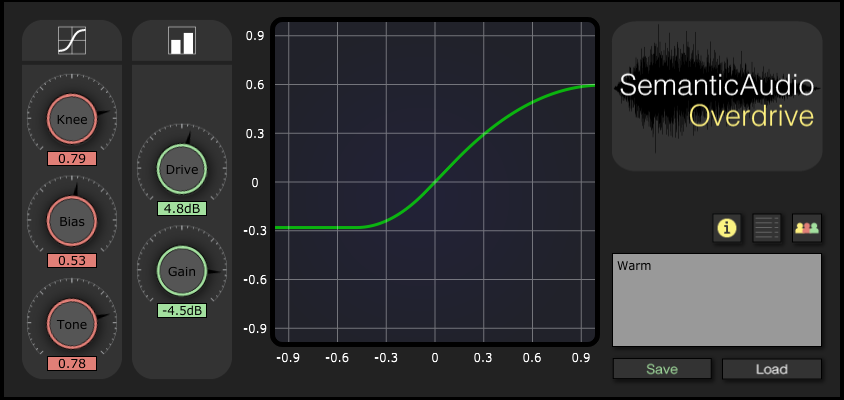
\includegraphics[width=0.8\textwidth]{chapter5/Images/SAFEDistortion.png}
				\caption{The Interface for the SAFE Distortion Plug-In}
				\label{fig:SAFE-Distortion}
			\end{figure}

			The LibXtract library \citep{bullock2007libxtract} is used in the analysis of the audio. Every
			scalar feature available within LibXtract is calculated along with the MFCCs and Bark Band
			Coefficients. In total five seconds of audio is analysed in frames of 4096 samples each.

			\note{Why 4096 samples? The real reason is because LibXtract works better that way. Will that cut
			the mustard?}

			One disadvantage in using plug-ins is that they cannot gather information about the rest of the
			processing chain they may be a part of. The timbral transformation the user is describing my be the
			result of several effects working together. This can be mitigated somewhat by asking users to
			describe only the effect the plug-in in question is providing.

			The SAFE plug-ins also suffer from the same issues other distributed tests do. The researcher
			forfeits control over the listening environment in order to gather results from a much larger sample
			of people. In fact the they provide even lest control that methodologies like that used in the
			Social EQ project \citep{cartwright2013socialeq} in that the choice of audio samples being used is
			decided by the test subject. 
